\documentclass[../main.tex]{subfiles}

\begin{document}
\section{Theory}
\subsection{Logistic regression}
Logistic regression is a method for classifying a set of input variables \ensuremath{\boldsymbol{x}} to an output or class \ensuremath{y_i, i=1,2, \ldots,K} where $K$ is the number of classes. The review in this section is based on Hastie et al. \cite[ch.~4]{HastieTrevor2009EoSL},  and the reader is referred to this book for a more detailed explanation of topic. The prediction of output classes which the input variables belongs to is based on the design matrix \ensuremath{\boldsymbol{X}\in\mathbb{R}^{n\times p}} that contains $n$ samples that each carry $p$ features. We distinct between \textit{hard} and \textit{soft classification}, which determines the input variable to a class deterministically or the probability that a given variable belongs in a certain class. The logistic regression model is given on the form
 
\begin{align}
    \begin{split}
        \log\frac{p(G=1|X=x)}{p(C=K|X=x)}&=\beta_{10}+\beta_1^Tx \\
        \log\frac{p(G=2|X=x)}{p(C=K|X=x)}&=\beta_{20}+\beta_2^Tx \\
        &\vdots\\ 
        \log\frac{p(G=K-1|X=x)}{p(C=K|X=x)}&=\beta_{(K-1)0}+\beta_{K-1}^Tx.
    \end{split}
\end{align}

We consider the binary, two-class case with \ensuremath{y_i \in [0,1]}. The probability that a given input variable $x_i$ belongs in class $y_i$ is given by the Sigmoid-function (also called logistic function):
\begin{align}
    p(x) = \frac{e^x}{1+e^x}=\frac{1}{1+e^{-x}}.
    \label{eq:sigmoid}
\end{align}

A set of predictors, \ensuremath{\boldsymbol{\beta}}, which we want to estimate with our data then gives the probabilities 

\begin{align}
    p(y_i=1|x_i,\boldsymbol{\beta})=\frac{\exp\left(\boldsymbol{\beta}^Tx_i\right)}{1+\exp\left(\boldsymbol{\beta}^Tx_i\right)} \\
    p(y_i=0|x_i,\boldsymbol{\beta})=1-p(y_i=1|x_i,\boldsymbol{\beta}).
\end{align} We define the set of all possible outputs in our data set \ensuremath{\mathcal{D}(x_i,y_i)}. Further, we assume that all samples \ensuremath{\mathcal{D}(x_i,y_i)} are independent and identically distributed. Now we can approximate the total likelihood for all possible outputs of \ensuremath{\mathcal{D}} by the product of the individual probabilities \cite[p.~120]{HastieTrevor2009EoSL} of a specific output $y_i$:

\begin{align}
    P(\mathcal{D}|\boldsymbol{\beta}) = \prod_{i=1}^n[p(y_i=1|x_i\boldsymbol{\beta})]^{y_i}[1-p(y_i=1|x_i,\boldsymbol{\beta})]^{1-y_i}.
    \label{eq:likelihood}
\end{align} We want to maximize this probability by using the maximum likelihood estimator (MLE). By taking the logarithm of \cref{eq:likelihood}, we obtain the log-likelihood in \ensuremath{\boldsymbol{\beta}}

\begin{align}
    \log P(\mathcal{D}|\boldsymbol{\beta}) = \sum_{i=1}^n[y_i\log p(y_i=1|x_i\boldsymbol{\beta})+(1-y_i)\log(1-p(y_i=1|x_i,\boldsymbol{\beta}))].
    \label{eq:log-likelihood}
\end{align}

By reordering the logarithms and taking the negative of \cref{eq:log-likelihood}, we obtain the \textit{cross entropy}

\begin{align}
    \mathcal{C}(\boldsymbol{\beta})=-\sum_{i=1}^n\left[y_i\boldsymbol{\beta}^Tx_i-\log\left(1+\exp\left(\boldsymbol{\beta}^Tx_i\right)\right)\right].
    \label{eq:cross-entropy}
\end{align} The cross entropy is used as our cost function for logistic regression. We minimize the cross entropy, which is the same as maximizing the log-likelihood, and obtain

\begin{align}
    \frac{\partial\mathcal{C}(\boldsymbol{\beta})}{\partial\boldsymbol{\beta}}=-\sum_{i=1}^nx_i(y_i-p(y_i=1|x_i,\boldsymbol{\beta}))=0.
\end{align} The second derivative of this quantity is

\begin{align}
    \frac{\partial^2\mathcal{C}(\boldsymbol{\beta})}{\partial\boldsymbol{\beta}\partial\boldsymbol{\beta}^T}=\sum_{i=1}^nx_ix_i^Tp(y_i=1|x_i,\boldsymbol{\beta})(1-p(y_i=1|x_i,\boldsymbol{\beta})).
\end{align} These expressions can be written more compactly by defining the diagonal matrix \ensuremath{\boldsymbol{W}} with elements \ensuremath{p(y_i=1|x_i,\boldsymbol{\beta})(1-p(y_i=1|x_i,\boldsymbol{\beta}))}, \ensuremath{\boldsymbol{y}} as the vector with our $y_i$s values and \ensuremath{\boldsymbol{p}} as the vector of fitted probabilities. We can then express the first and second derivatives in matrix form

\begin{align}
    \frac{\partial\mathcal{C}(\boldsymbol{\beta})}{\partial\boldsymbol{\beta}}&=-\boldsymbol{X}^T(\boldsymbol{y}-\boldsymbol{p}) \\
    \frac{\partial^2\mathcal{C}(\boldsymbol{\beta})}{\partial\boldsymbol{\beta}\partial\boldsymbol{\beta}^T} &= \boldsymbol{X}^T\boldsymbol{W}\boldsymbol{X},
\end{align} also known as the Jacobian and Hessian matrices, respectively. We will use the stochastic gradient descent (SGD) (\cref{sec:sgd}) to find the optimal parameter \ensuremath{\boldsymbol{\beta}}. 

\subsection{Stochastic Gradient Descent}\label{sec:sgd}
\textit{Gradient descent} describes the process of finding a local minimum of a function (the cost function, in our case) by following the negative value of the gradient at each point, stepwise. \textit{Stochastic gradient descent} or SDG is a way of increasing the numerical efficiency of this process, by doing this process stochastically.

This involves randomly dividing the training data into a given number of \textit{mini batches}. For each mini batch, the gradient is found by averaging the gradient value each mini batch sample has. Then the weights and biases are updated (take a step down the "slope") and the process is repeated for the rest of the mini batches. The updating done at each mini batch is expressed mathematically as

\begin{align*}
    w&\rightarrow w' = w - \frac{\eta}{m}\sum_i^m \nabla C_{i,w} \\
    b&\rightarrow b' = b - \frac{\eta}{m}\sum_i^m \nabla C_{i,b},
\end{align*}

where $m$ is the number of data points in the mini batches and $\nabla C_i$ is the gradient of the cost function at each individual data point. After exhausting all the training data, we have finished a so-called \textit{epoch}, of which we can perform as many as necessary.

\subsection{Convolutional neural network (CNN)}
In deep learning, a convolutional neural network (CNN), is a specialized kind of neural network most commonly applied to analyzing images. Convolutional networks can be thought of as neural networks that use convolution in place of a general matrix multiplication in at least one of their layers \cite{Goodfellow-et-al-2016}. 

In this section we assume that you are already familiar with the multilayer perception (MPL). If you wish to refresh your memory you can look into our previous work on MPL \cite{project2}. %first give motivation, then describe a simple cnn for image classification architecture ...

\subsubsection{Motivation}
For each layer in the MPL we have to perform a matrix multiplication of the activation's, $a^l$ with the new weights, $w^l$. As an example we consider an image size of \ensuremath{28\times28\times3} (28 pixels wide, 28 pixels high, 3 color channels). A single fully-connected neuron in the first hidden layer of the MPL would then have \ensuremath{28\times28\times3=2352} weights. This amount of operations is manageable and might perform well for basic binary images, but does not scale to a high pixelated image of size \ensuremath{M\times N\times3}.

Further, MPLs ignore the information brought by pixel position and correlation with neighbour pixels. Another drawback is that MPLs are not translation invariant. If an element of interest appear in the top left of the image in one picture and the bottom right of another picture, the MPL will try to correct itself and assume that the element will always appear in this section of the image. 

The CNN successfully captures the spatial and temporal dependencies through the application of relevant filters. A better fit to the image dataset is obtained by the reduction in the number of parameters involved and the reusability of weights. Another advantage of convolution is that it provides a mean for working with inputs of variable size. In the following we describe a simple CNN architecture for image classification. 

\begin{figure}[!htb]
    \centering
    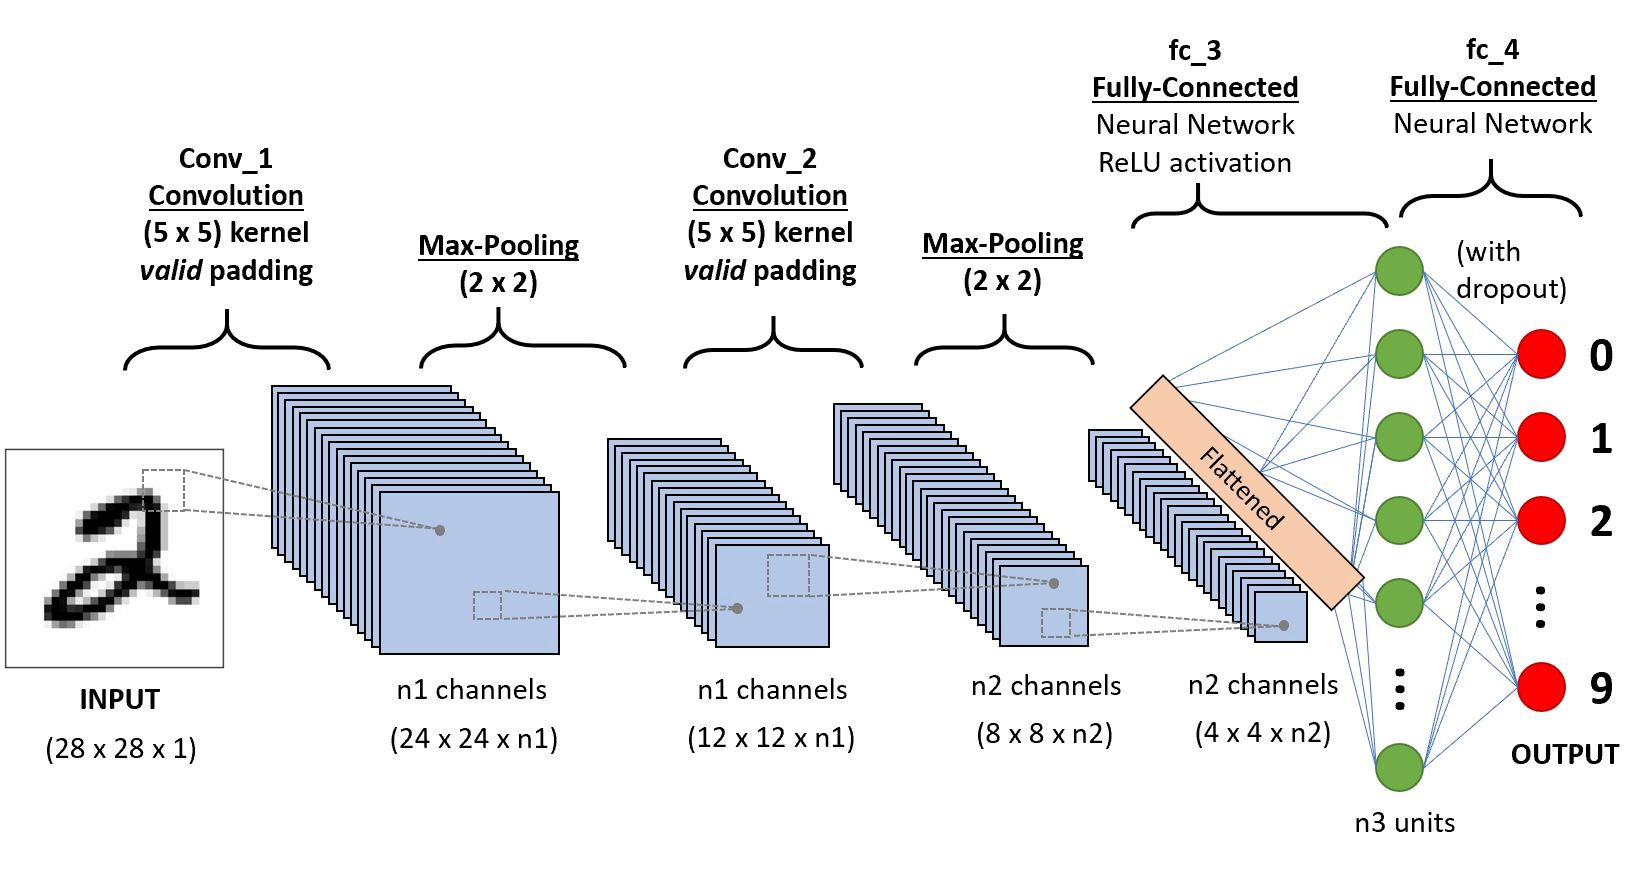
\includegraphics[width=\textwidth]{fig/ex-cnn.jpeg}
    \caption{An example of a CNN architecture to classify handwritten digits. Figure taken from \cite{sumit2018}.}
    \label{fig:example-cnn}
\end{figure}

\subsubsection{Input layer}
The first layer is the \textit{input layer}. This layer will hold the raw pixel values of the image to be studied. In the case of a RGB color image we have three pixel grids representing red, green and blue. The number of pixel grids is referred to as the image \textit{depth}. A RGB image thus have a depth of three and a grayscale image has a depth of one. \Cref{fig:rgb-input} show an example of a \ensuremath{4\times4\times3} RGB image. 

\begin{figure}[!htb]
    \centering
    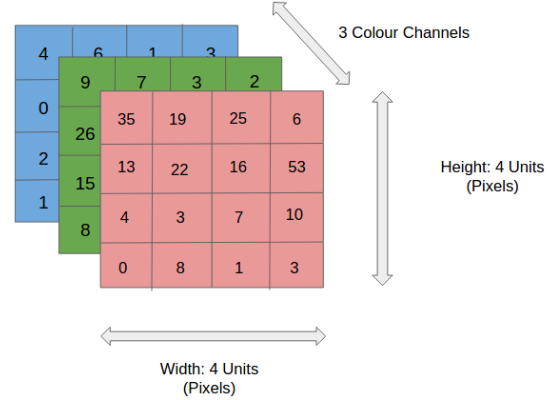
\includegraphics[width=0.8\textwidth]{fig/rgb.png}
    \caption{An example of an \ensuremath{4\times4\times3} RGB image. Figure taken from \cite{sumit2018}.}
    \label{fig:rgb-input}
\end{figure} 

\subsubsection{Convolution layer}
The main purpose of the \textit{convolution layer} is to relate pixels to each other spacially. Here, the element involved in carrying out the convolution operation is reffered to as a \textit{filter} or \textit{kernel (K)}. The kernel matrix typically has shape \ensuremath{3\times3} or \ensuremath{5\times5} and has the depth of the input image.

The filter starts in the upper left corner, the algorithm looks at a section of the input layer \ensuremath{(I_n)} that has the same shape as $K$. It then performs a matrix multiplication between $I_n$ and $K$ and the results are summed with the bias to give a squashed one-depth channel convoluted feature output \cite{sumit2018}. Then, the filter moves to the right by an amount referred to as the \textit{stride length} till it parses the complete width of the image. Moving on, the filter hops down to the leftmost section of the image with the same stride value. The process is repeated until the entire image is traversed. 

\begin{figure}
    \centering
    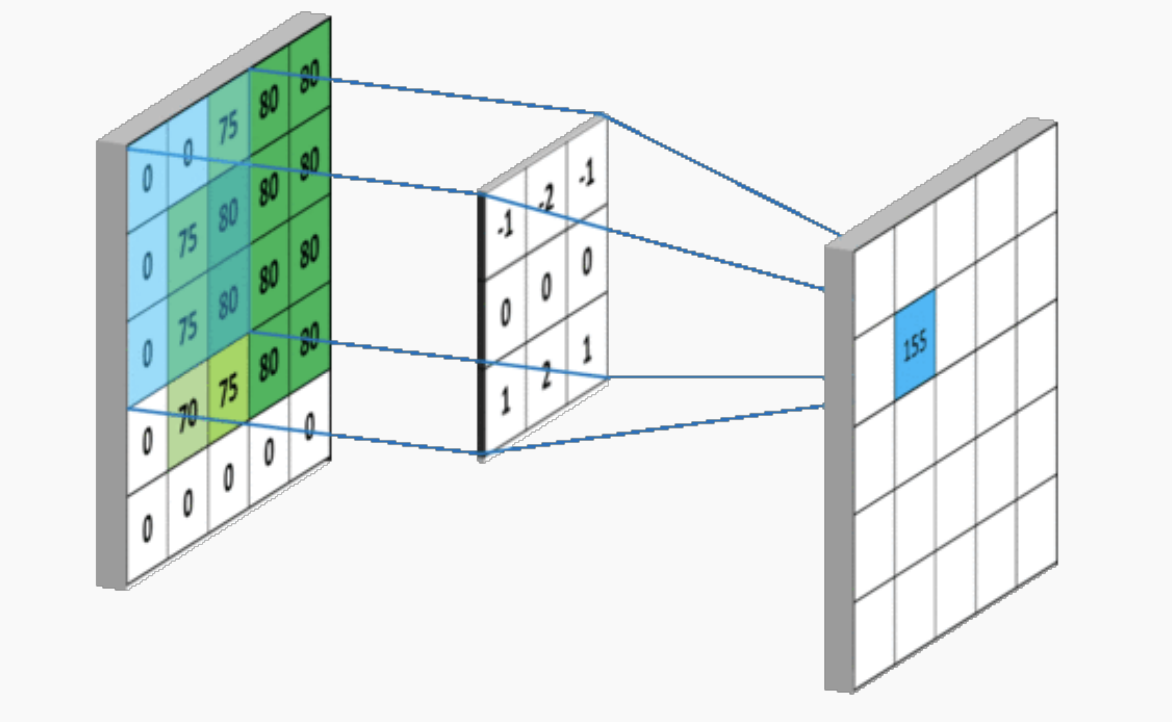
\includegraphics[width=0.7\textwidth]{fig/convolution.png}
    \caption{An example of how a convolution layer is applied to a image using kernel filters. Figure taken from \cite{stewart2019}.}
    \label{fig:convolution}
\end{figure}

The convolution layer reduces the size of the input. For a \ensuremath{5\times5} input with stride length 1, such as the example in \cref{fig:convolution}, will result in a \ensuremath{3\times3} convoluted feature output. If this is not desirable, we can use \textit{padding}. \textit{Same padding} involves adding a layer or several layers of pixels of value 0 around the entire input. The input is now a \ensuremath{6\times6} matrix, and the convoluted feature output will have size \ensuremath{5\times5}. If the stride length is larger than 1, \textit{valid padding} can be used to make the size of the convoluted feature output less reduced. In a typical CNN architecture, both valid and same padding is used. 

\subsubsection{ReLU layer}
The \textit{ReLU layer} applies the non-saturating activation function \ensuremath{f(x)=\text{max}(0,x)}. This activation function effectively removes negative values from an activation map. this leaves the size of the volume unchanged. Further, it increases the nonlinear properties of the decision function and of the overall network without affecting the receptive fields of the convolution layer \cite{wiki:xxx}.  

\subsubsection{Pooling layer}
The \textit{pooling layer} is used to non-linearly downsample a activation map. Pooling utilizes the idea that the exact location of a feature is less important than a rough estimate of the relative location of other features. When the spatial dimension is reduced, forcing translation invariance, overfitting and the amount of computations needed is reduced. The pooling map sizes are typically \ensuremath{2\times2}, larger sizes may also be used. In the following we consider a pooling size of \ensuremath{2\times2}. Pooling may compute a max or an average from the portion of the image covered by the Kernel, see the example in \cref{fig:pooling}. Max pooling is better at reducing noise, and will therefore typically perform better. For large images it is typical to resend the feature through convolution and pooling layers several times, this comes with a increased computational cost. 

\begin{figure}
    \centering
    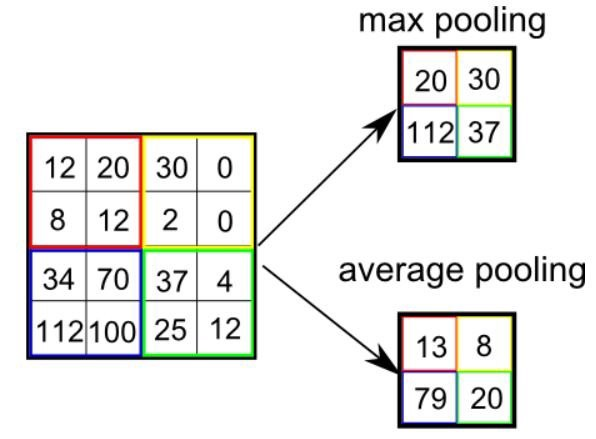
\includegraphics[width=0.6\textwidth]{fig/pooling.jpeg}
    \caption{Two types of pooling: computing a max or an average from the portion of the image covered by the Kernel. Figure taken from \cite{sumit2018}.}
    \label{fig:pooling}
\end{figure}

\subsubsection{Fully-connected layer and output layer}
Finally, after several convolutional and pooling layers, we have the \textit{fully-connected} layer (FCL). Here, the input is first flattened before it is sent through a traditional feed-forward neural network layer (FFNN). There are typically several FCLs and the final layer is referred to as the \textit{output layer}. Backpropagation is applied to every iteration of training, and over a series of epochs, the algorithm is able to classify images. %using the softmax classification technique?? 

\subsection{Quality of models}
We measure the performance of the different models used in this work. For classification, we measure how accurate the predictions given by the model are by the so called accuracy score. The accuracy score is given by

\begin{align}
    \text{accuracy}=\frac{1}{n}\sum_{i=0}^nI(t_i=y_i),
    \label{eq:accuracy-score}
\end{align}

where $n$ is the number of samples, $t_i$ represents the target output and $I$ is the indicator function, which returns 1 if \ensuremath{y_i=t_i} and 0 otherwise. 

The \textit{confusion matrix} of a categorical predictor is a table layout that presents a more in-depth view of the method performance than the accuracy score. Each row of the matrix represents the instances in a predicted class while each column represents the instances in an actual class. The advantage of the confusion matrix is that it better illustrates the misclassified instances. Below, we illustrate the confusion matrix for the three-class A, B and C:

\begin{table}[htb]
    \centering
    \begin{tabular}{c c | c c c}
    
     &&  & True & \\
     && A & B & C \\
    \midrule
    &A& AA & AB & AC\\
    Pred & B & BA & BB & BC\\
    &C& CA & CB & CC\\
 

    \end{tabular}
    \label{tab:confusion-matrix}
 \end{table}

All the correct predictors are located in the diagonal of the table, while the non-diagonal elements represent the misclassificatons of the predictors. 

\end{document}